\section{Natural clouds}

\subsection{Formation}
Clouds, as seen in nature, consist of of a visible body of tiny water droplets and frozen crystals. 
In their natural occurence, clouds are mostly generated from a nearby source of moisture, usually in the form of water vapor. 
This composition of particles creates the pleasant look of a white-grayish "fluffy" mass, floating in the sky.
\\
Due to certain factors like altitude or water source, different types of cloudscapes can be formed. They vary in shape, \gls{convection}, density and more.
That makes different cloudscapes highly unique in terms of appearance.
\\
For now, those factors are regarded as nature's randomness. However, an approximation of randomness will be covered in section \sectionref{section:noise_generation}.


\subsection{Types of clouds}
\label{section:cloud-types}
Cloudscapes are classified in multiple groups, mainly differing depending in their altitude, meaning the distance from the earth's surface to the cloud formation.
The following four cloud genera stand out due to their distinctiveness. A realistic simulation of a cloud system would consist of a combination of these types, which is why they are displayed here.
\begin{figure}[ht]
    \centering
        \begin{minipage}{0.47\linewidth}
            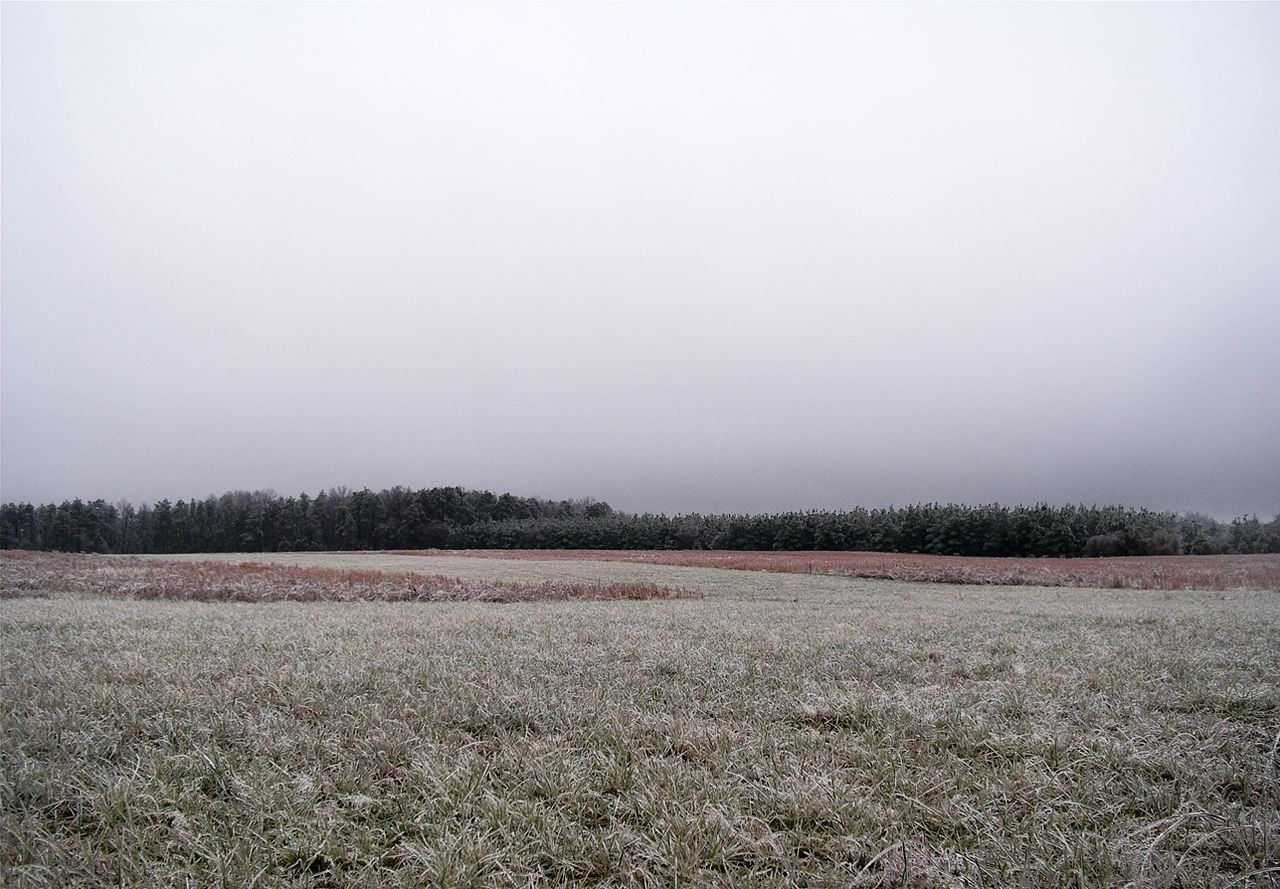
\includegraphics[width=\linewidth]{cloudforms-stratus}
            \captionof{figure}{Photographic reference of stratus clouds\protect\cite{img:cloudforms:stratus}.}
            \label{img:photo:cloudforms-stratus}        
        \end{minipage}        
    \hfill
        \begin{minipage}{0.47\linewidth}
            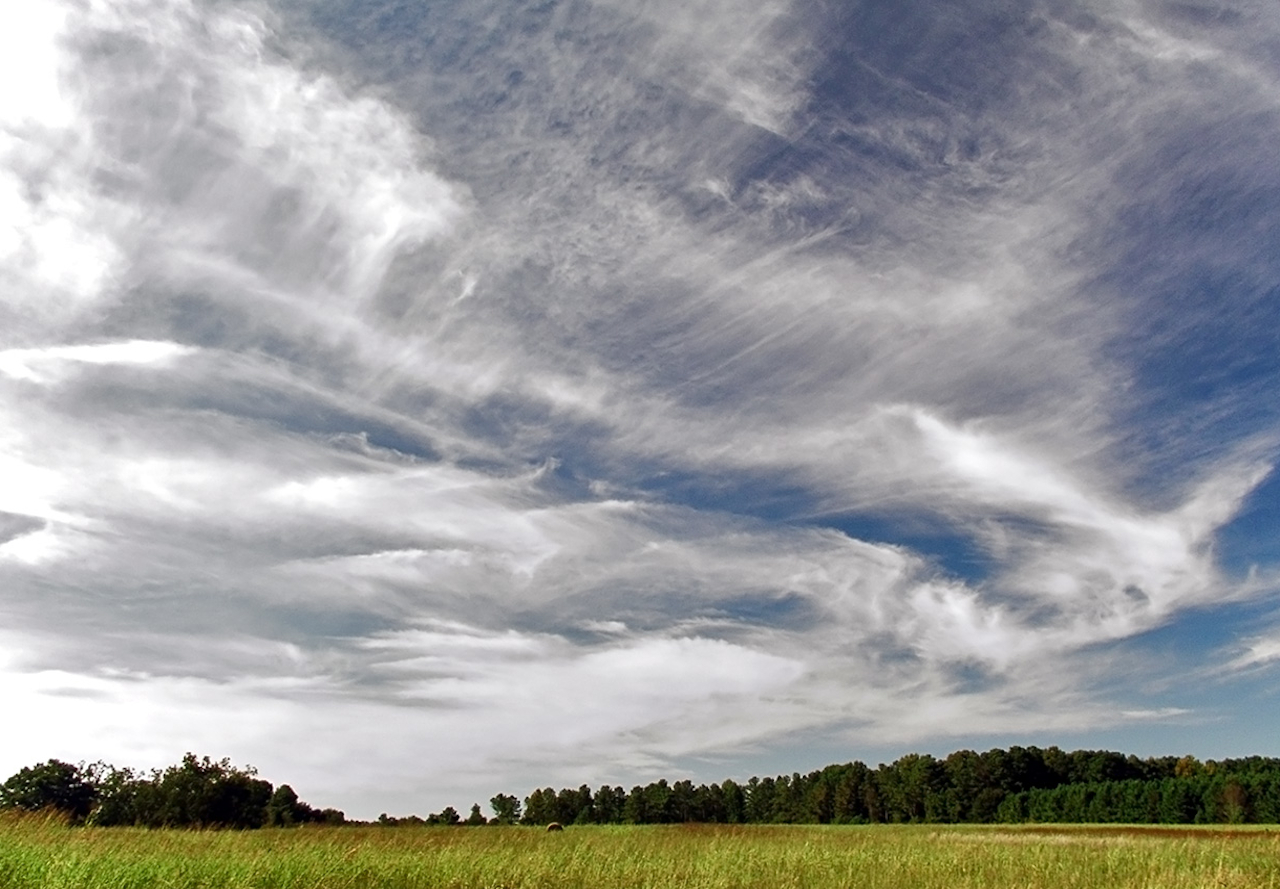
\includegraphics[width=\linewidth]{cloudforms-cirrus}
            \captionof{figure}{Photographic reference of cirrus clouds\protect\cite{img:cloudforms:cirrus}.}
            \label{img:photo:cloudforms-cirrus}        
        \end{minipage}
\end{figure}

\begin{figure}[ht]
    \centering
        \begin{minipage}{0.47\linewidth}
            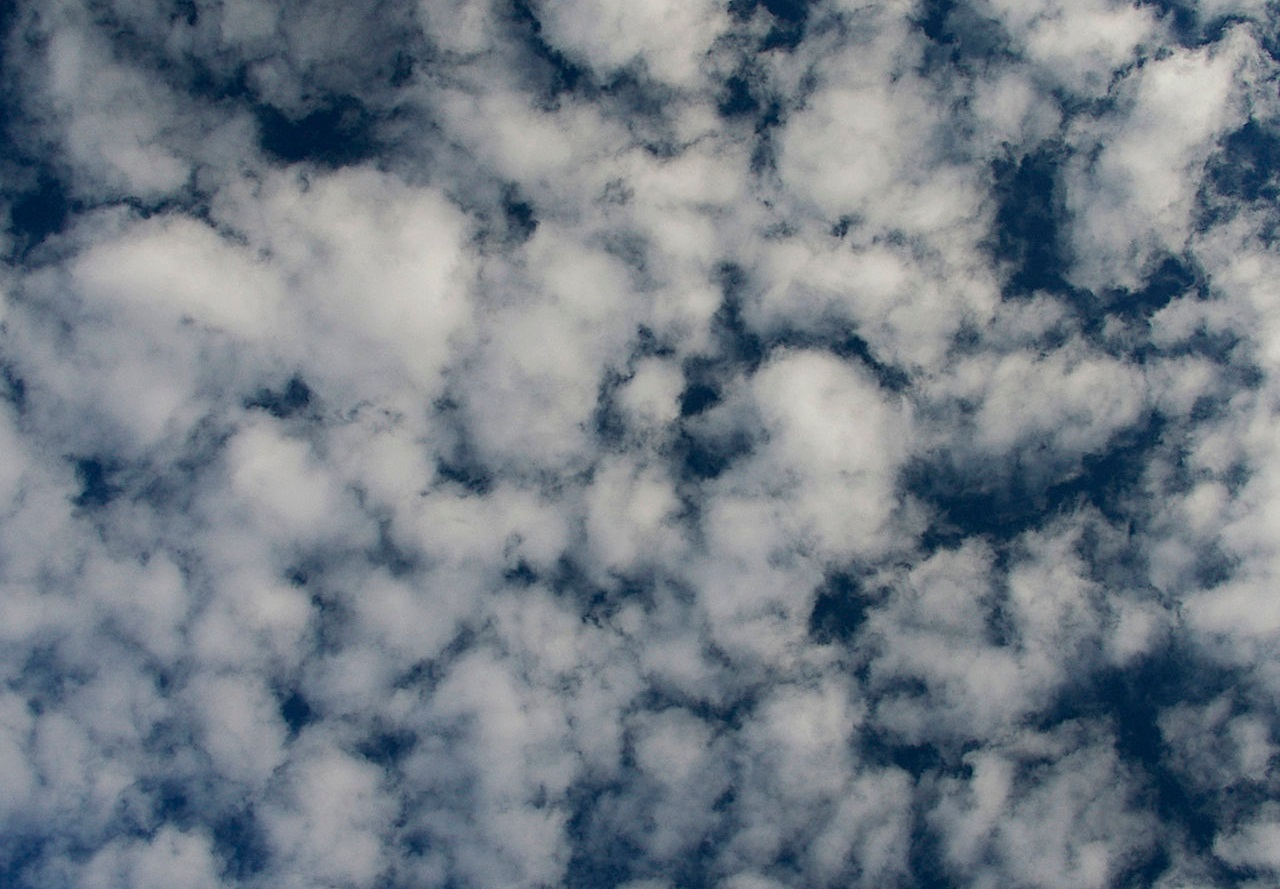
\includegraphics[width=\linewidth]{cloudforms-altocumulus}
            \captionof{figure}{Photographic reference of an altocumulus cloud formation\protect\cite{img:cloudforms:altocumulus}.}
            \label{img:photo:cloudforms-altocumulus}        
        \end{minipage}        
    \hfill
        \begin{minipage}{0.47\linewidth}
            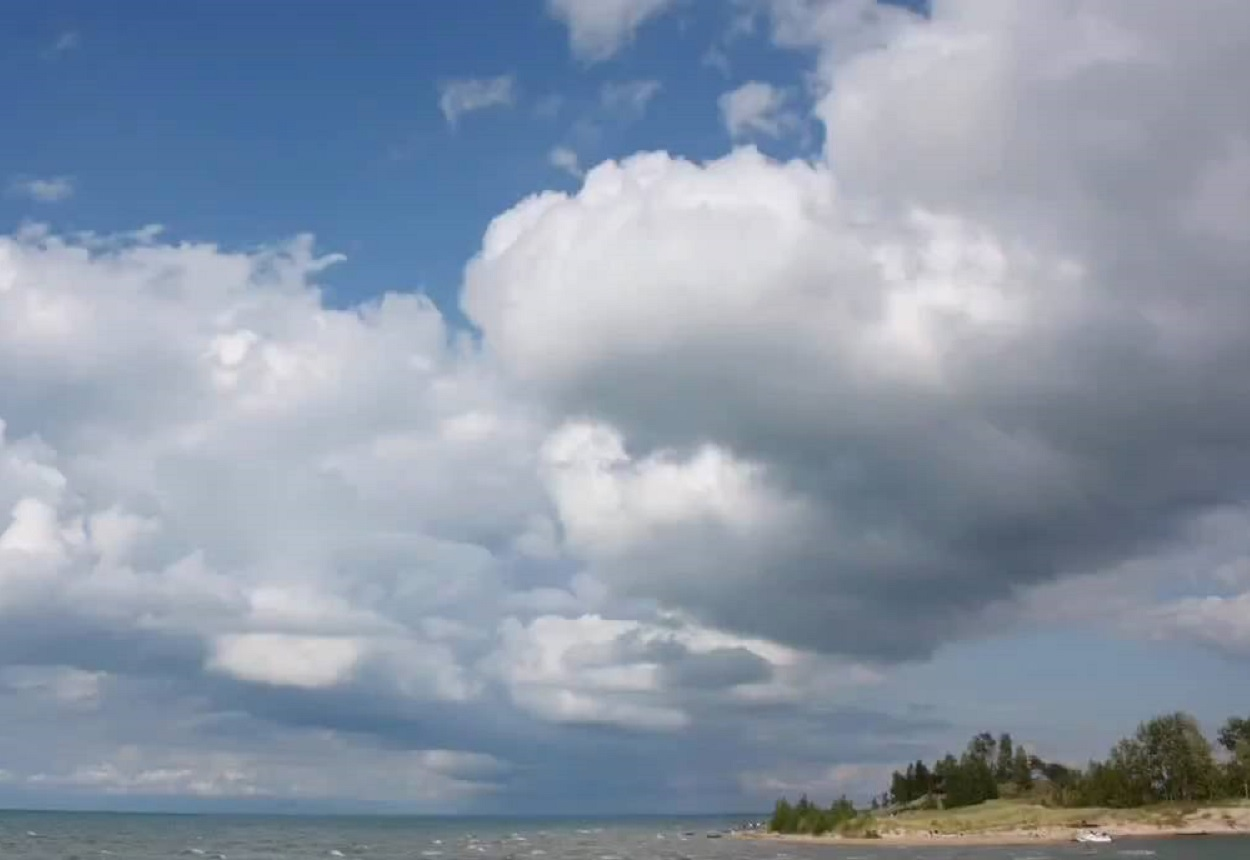
\includegraphics[width=\linewidth]{cloudforms-stratocumulus}
            \captionof{figure}{Photographic reference of stratocumulus cloudscape\protect\cite{img:cloudforms:stratocumulus}.}
            \label{img:photo:cloudforms-stratocumulus}        
        \end{minipage}  
\end{figure}



\subsection{Clouds in games}
Depicted in \autoref{img:photo:cloudforms-altocumulus} and \autoref{img:photo:cloudforms-stratocumulus} of \sectionref{section:cloud-types} are clouds of the genus \textit{cumulus}, which translated to English means \textit{heap} or \textit{pile}.
Their distinctive cotton-like look makes them easy to recognize, which is also why they are often used in games as a reference for "normal" clouds. 
\\
In games, the formation as well as the composition of clouds are irrelevant, as they are essentially only used for cinematic ambience or as a medium to enhance the atmosphere. This leaves just the rendering technique to worry about.

\subsubsection{Rendering techniques}
A widespread solution for rendering clouds in games is not rendering them separately at all, but instead using a set of polar sky dome images, also known as the skybox. This is a six-sided cube which is rendered around the whole game world. On each inward looking face of the cube, one of the sky dome images is rendered, creating a seemless sky around the complete box.

\begin{figure}[ht]
    \centering
        \begin{minipage}{0.47\linewidth}
            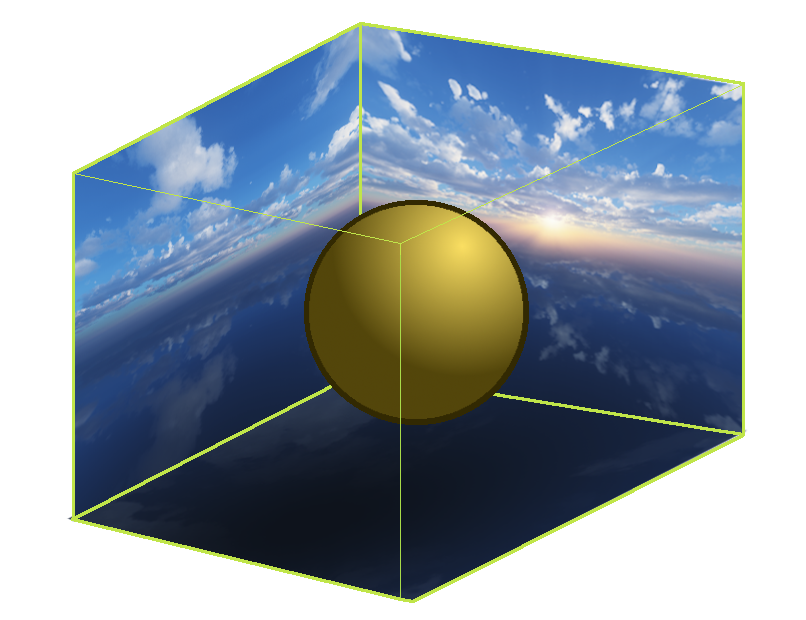
\includegraphics{edits/skybox}
            \captionof{figure}{Three sides of a six-sided skybox cube and a ball representing the game world}
            \label{img:edits:skybox}            
        \end{minipage}        
    \hfill
        \begin{minipage}{0.47\linewidth}
            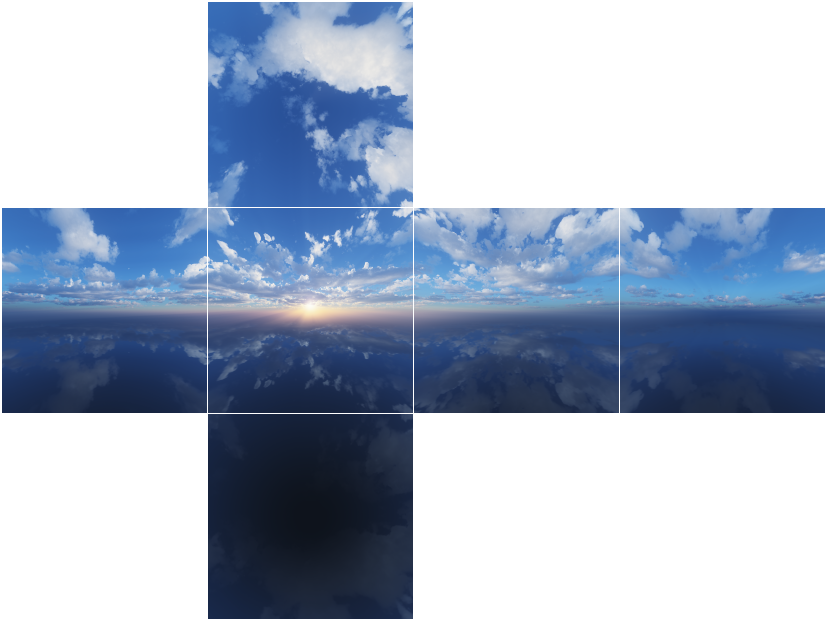
\includegraphics[width=\linewidth]{edits/skybox_layedout}
            \captionof{figure}{Photographic reference of stratocumulus cloudscape\protect\cite{img:cloudforms:stratocumulus}.}
            \label{img:edits:skybox_layedout}        
        \end{minipage}  
\end{figure}




\begin{figure}[ht]
    \centering
    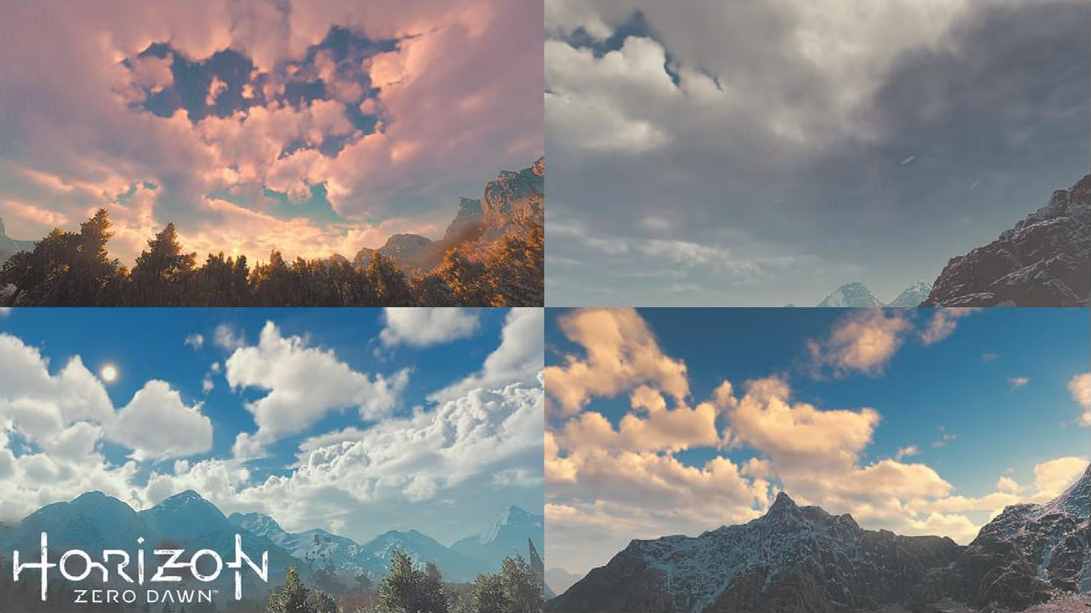
\includegraphics[width=\linewidth]{rendered-clouds-zerodawn}
    \captionof{figure}{Several volumetric cloudscapes from the game \textit{Horizon: Zero Dawn}, drawn in real time\protect\cite{img:rendered:clouds-zerodawn}.}
    \label{img:rendered:clouds-zerodawn}        
\end{figure}